\chapter{Elementi Base}
\label{ch:second_chapter}

In questo capitolo ci saranno esempi base di elenchi puntati, figure, tabelle, formule, algoritmi e codici.

\bigskip
\noindent Esempio di elenco puntato:
\begin{itemize}[noitemsep]
    \item \textbf{primo punto in grassetto}; % in grassetto
    \item secondo punto, se preferisci che non sia in grassetto;        % se lo preferisci senza grassetto
\end{itemize}

\section{Sezione nel Secondo Capitolo}
\label{sec:id}

Esempio di immagine in Figura \ref{fig:uno}. Ricorda di menzionare sempre nel testo, usando \textbackslash ref, tutte le figure/tabelle/algoritmi/codici che inserisci. \footnote{Un'esempio di come aggiungere una footnote, spesso magari usata per citare o riportare qualche sito, come tipo~\url{https://ditto.ing.unimore.it/}\hspace{2pt}\raisebox{-0.4\height}{},}
    
\begin{figure}[H] % Starts the figure environment. [htbp] suggests placement: Here, Top, Bottom, Page.
    \centering % Centers the image and caption horizontally on the page.
    
    % \includegraphics[options]{filename} is the core command to insert the image.
    % --- Options ---
    % 'width=\linewidth': Makes the image take up the full width of the text area.
    %                  Other options: 'width=8cm', 'scale=0.5' (half size),
    %                  'height=5cm', 'angle=90' (rotate by 90 degrees).
    % 'keepaspectratio': Very important! Prevents distortion when setting both width and height.
    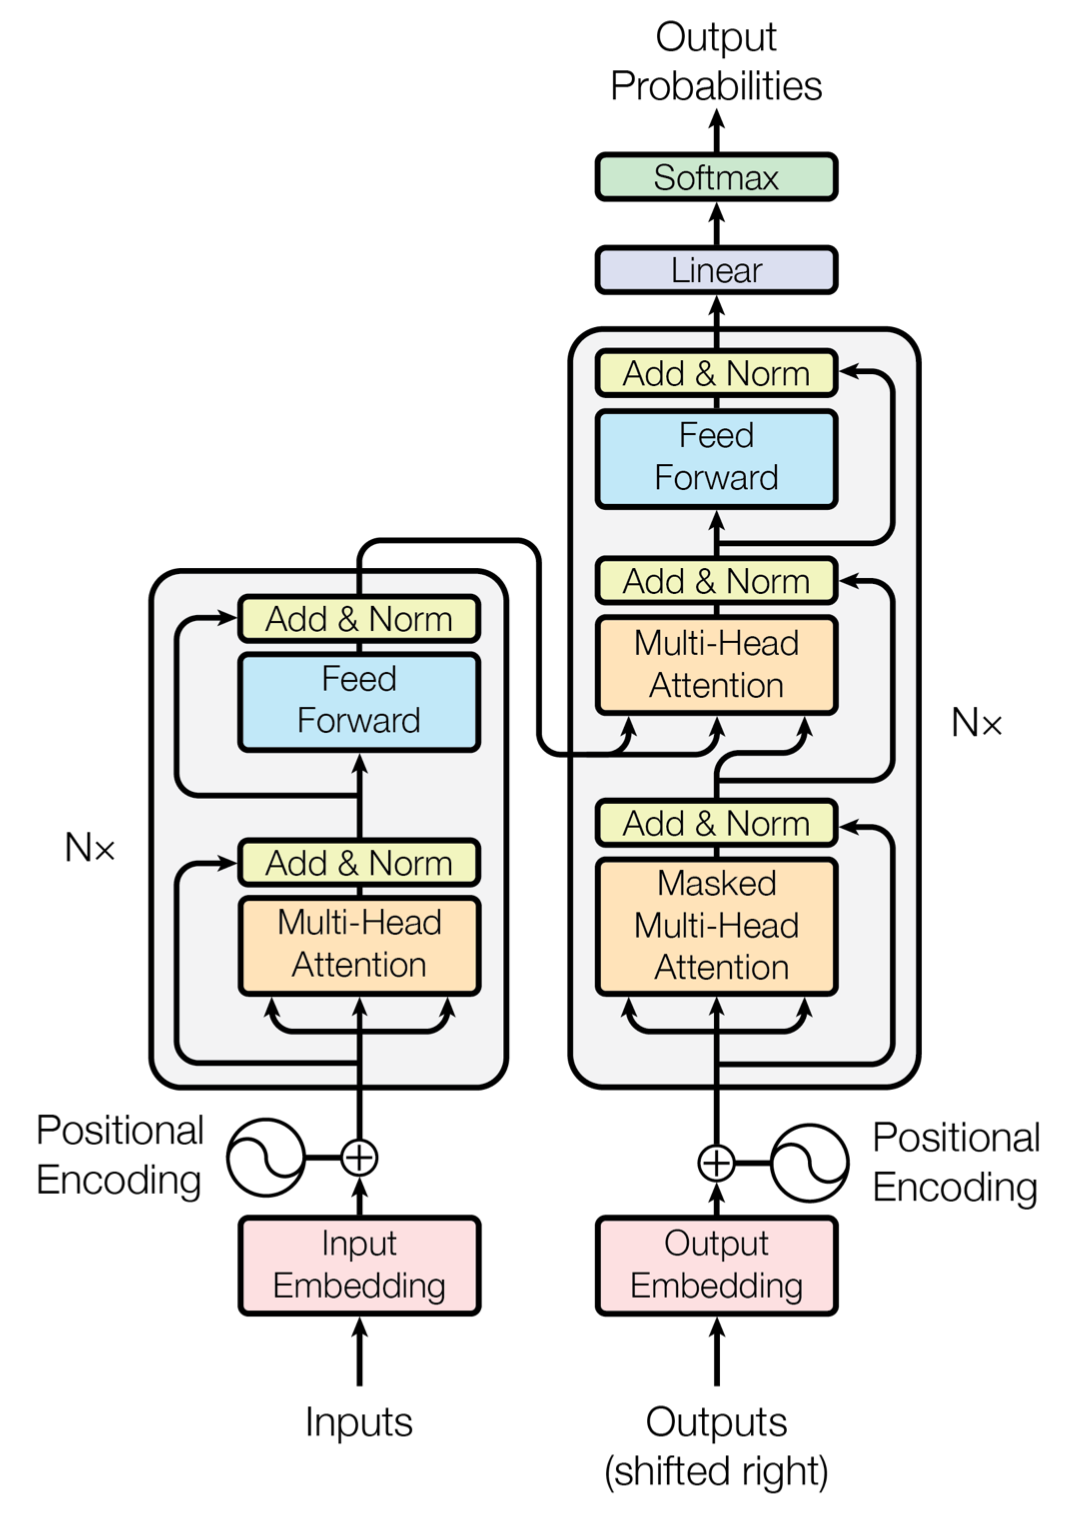
\includegraphics[width=0.8\linewidth, keepaspectratio]{images/architetture/t.png} % Replaced with a placeholder image command for demonstration.
    % In a real document, you'd put the actual filename: \includegraphics[width=0.8\linewidth]{my_photo.png}
    
    \caption{L'architettura introdotta da Vaswani nel famoso Paper  \textit{"Attention is All You Need"}~\cite{vaswani2017attention}.} % The caption appears below the image.
    \label{fig:uno} % Label for referencing this figure (e.g., "see Figure \ref{fig:sunset_image}").
\end{figure}

\section{Un'Altra Sezione nel Secondo Capitolo}
Esempio di una tabella con relativa citazione, Tabella~\ref{tab:table_example}.

\begin{table}[tb] % Inizio ambiente tabella flottante; [tb] = top o bottom della pagina
\centering % Centra la tabella
\caption{Esempio di tabella con vari campi, spunte e croci.} % Didascalia
\begin{adjustbox}{width=0.9\textwidth} % Adatta la tabella al 90% della larghezza del testo
{\normalsize % Imposta la dimensione normale del font
\setlength{\tabcolsep}{8pt} % Imposta la spaziatura orizzontale tra le colonne

\begin{tabular}{cccrrrr} % Crea una tabella con 7 colonne:
                         % c = allineamento centrato, r = allineamento a destra
\toprule % Riga orizzontale superiore spessa (booktabs)

% \makecell permette di inserire testo formattato o su più righe all’interno di una cella.
% È utile soprattutto nelle intestazioni per evitare l’uso di \parbox o \multicolumn.
% Qui viene usato per centrare e rendere in grassetto il testo delle intestazioni.
\makecell[c]{\textbf{Frutto}} & 
\makecell[c]{\textbf{Arancione}} & 
\makecell[c]{\textbf{Si sbuccia}} & 
\makecell[c]{\textbf{Peso}} &   
\makecell[c]{\textbf{Prezzo}} &   
\makecell[c]{\textbf{Zucch.}} &   
\makecell[c]{\textbf{Voto (1–10)}} \\  
% Il simbolo & separa le colonne all'interno di una riga.
% Ogni cella di una riga è delimitata da un &.
% Il comando \\ indica la fine della riga e l’inizio di una nuova.
\midrule % Riga orizzontale media

Arancia & \checkmark  & \checkmark & 0.200 & 2.50 & 9.0 & 8 \\ % Esempio di riga: & separa le colonne, \\ chiude la riga
Mandarino & \checkmark & \checkmark & 0.120 & 3.20 & 8.5 & 9 \\
Limone & \ding{55} & \checkmark & 0.100 & 3.50 & 2.5 & 6 \\
\midrule

Mela & \ding{55} & \ding{55} & 0.180 & 2.80 & 10.0 & 8 \\
Banana & \ding{55} & \checkmark & 0.150 & 1.10 & 12.2 & 9 \\
Kiwi & \ding{55} & \checkmark & 0.120 & 4.00 & 9.1 & 7 \\
Mango & \checkmark & \checkmark & 0.300 & 5.00 & 14.0 & 10 \\
\bottomrule % Riga inferiore spessa

\end{tabular} % Fine ambiente tabular
} % Fine del blocco \normalsize
\end{adjustbox} % Fine dell’adattamento di larghezza
\label{tab:table_example} % Etichetta per riferimenti
\vspace{-10pt} % Riduce lo spazio sotto la tabella
\end{table} % Fine ambiente tabella
 % input command can help to get a clearer and more readable latex code, in this case we moved the table inside another file

\section{Formule Matematiche}
Qui due esempi di come fare formule matematiche, come riconoscerete bene in Eq.~\ref{eq:continuous_ft} abbiamo la versione integrale della Trasformata di Fourier mentre in Eq.~\ref{eq:discrete_ft} ne abbiamo la formulazione discretizzata con la sommatoria.

% --- Formula 1: Continuous Fourier Transform (The Integral) ---
\begin{equation}
    \label{eq:continuous_ft}
    % \int is the integral symbol. 
    % _{...} is the lower limit (subscript).
    % ^{...} is the upper limit (superscript).
    X(f) = \int_{-\infty}^{\infty} x(t) e^{-j 2\pi f t} \, dt
\end{equation}


% --- Formula 2: Discrete Fourier Transform (The Summation) ---
\begin{equation}
    \label{eq:discrete_ft}
    % \sum is the large Sigma symbol for summation.
    % We use x_n to denote the n-th item in the sequence (subscript n).
    X_k = \sum_{n=0}^{N-1} x_n \cdot e^{-i \frac{2\pi}{N} k n}
\end{equation}

\section{Esempio di Algoritmo }
Nell'Algoritmo \ref{alg:dijkstra} si può vedere un modo per ottenere il cammino minimo.

\begin{algorithm}[H] % H per forzare il posizionamento esattamente in questa posizione. E' sconsigliato usarlo sempre.
\caption{Dijkstra's Algorithm} % Title of the algorithm
\label{alg:dijkstra} % Label for referencing (e.g., "see Algorithm \ref{alg:dijkstra}")

    \begin{algorithmic}[1] % The [1] means "number every single line"
        
        % \Procedure{Name}{Arguments} creates the function header
        \Procedure{Dijkstra}{$G, s$} 
            
            % \State is used for every standard line of code
            \State $dist[] \gets \infty$ \Comment{Initialize distances to infinity}
            \State $dist[s] \gets 0$     \Comment{Distance to source is 0}
            \State $Q \gets V[G]$        \Comment{Add all nodes to the queue}
            
            % \While{condition} automatically handles indentation and the "do" keyword
            \While{$Q$ is not empty} 
                \State $u \gets$ vertex in $Q$ with min $dist[u]$
                \State remove $u$ from $Q$
                
                % \For{condition} loop
                \For{each neighbor $v$ of $u$} 
                    \State $alt \gets dist[u] + length(u, v)$
                    
                    % \If{condition} block
                    \If{$alt < dist[v]$} 
                        \State $dist[v] \gets alt$
                        \State $prev[v] \gets u$
                    \EndIf % You must explicitly close the If
                    
                \EndFor % You must explicitly close the For
            \EndWhile % You must explicitly close the While
            
            \State \textbf{return} $dist[], prev[]$
            
        \EndProcedure % Ends the function
        
    \end{algorithmic}
\end{algorithm}

\section{Esempi di Codice}
Puoi anche includere alcuni esempi di codice, purché non siano troppo lunghi. Un esempio di può vedere nel Codice \ref{cod:hello}
\begin{lstlisting}[caption={Codice di esempio, tratto da helloworldspam.py}, label={cod:hello}]
print('Starting the ultimate hello world spammer')
for i in range(10000000):
    print("Hello, world!")
\end{lstlisting}

\section{Gestione della Bibliografia}
Tutti i riferimenti bibliografici andranno inseriti nel file ``.bib'' del progetto. In questo template il file è ``bibliography.bib''. Per citare un riferimento occorre usare il comando ``\textbackslash cite\{<id>\}'', come ad esempio \cite{vaswani2017attention}.